\documentclass[11pt]{article}
\usepackage{scicite}
\usepackage{times}
\topmargin 0.0cm
\oddsidemargin 0.2cm
\textwidth 16cm 
\textheight 21cm
\footskip 1.0cm
\newenvironment{sciabstract}{%
\begin{quote} \bf}
{\end{quote}}
\renewcommand\refname{References and Notes}
\newcounter{lastnote}
\newenvironment{scilastnote}{%
\setcounter{lastnote}{\value{enumiv}}%
\addtocounter{lastnote}{+1}%
\begin{list}%
{\arabic{lastnote}.}
{\setlength{\leftmargin}{.22in}}
{\setlength{\labelsep}{.5em}}}
{\end{list}}



\title{Reflections of Evaluation for Clustering and Machine Translation} 
\author{
Jo\~{a}o Sedoc \\
Department of Computer Science\\
University of Pennsylvania\\
Philadelphia, PA 19104 \\
\texttt{joao@cis.upenn.edu}
}

\date



%%%%%%%%%%%%%%%%% END OF PREAMBLE %%%%%%%%%%%%%%%%



\begin{document} 

% Double-space the manuscript.

\baselineskip24pt

% Make the title.

\maketitle 

\begin{sciabstract}
  This paper presents a short summary of the insights that I gleaned from Ani Nenvoka's class
  on evaluation in Spring 2015.
The fundamental goal of evaluation is to make inferences. Evaluation is should {\it not} be a beat state-of-the-art but instead one should carefully select an experiment that tests both the validity and impact of a new method, application or dataset.
  This paper is not a full summarization of all of the articles read in class, but instead I highlight some of what I consider the key concepts and take aways from this class.
\end{sciabstract}



\section*{Introduction}
  This paper is also intended to serve two purposes, the first being to satisfy the paper requirement and more importantly the second which is more for myself in the future.
  The class syllabus states
\begin{quote}
The topic for cis 630 this year is``Evaluation methodology for NLP''. NLP is an empirical discipline and practically all published papers contain an evaluation section in which the authors quantify how good is their proposed method. The results are the basis for the scientific conclusions that can be drawn about the problem, which expand our knowledge in a particular area of research. The goal of the course if to establish how to define a good evaluation score, how to apply it in evaluation and most importantly, how to use scores to make meaningful scientific conclusions. 
\end{quote}

So how do we properly evaluate different methods and papers? Messick \cite{messick1995validity} argues that evaluation has six fundamental characteristics: 
content, substantive, structural, generalizability, external,
and consequential aspects of construct validity. 
For natural language processing (NLP) we are mostly concerned with content, structural and generalizability. 

Content is merely the coverage of the test in order to make sure that proper evaluation of topic is covered. While this is obvious for evaluating human knowledge it is far to often forgotten. In numerous papers that we read there is a divorce between evaluation metric / task and model. 

By structural Messick means
``theoretical rationales
for the observed consistencies in test responses'' \cite{messick1995validity}. What is the theoretical foundation behind the model and do we have theoretical foundations behind the model and evaluation task and metric. Often in statistics and to a lesser extent in machine learning we start with the model or metric and then find an application. In this instance theoretical evaluations based off of mathematical formulae or synthetic data are valuable. However, for the NLP community there is very little focus on theoretical foundations for evaluation. In the NLP community we do not have a large tradition of synthetic data. Model evaluation is much easier. I believe that we should mimic some of the properties of the real dataset. Note that for training and evaluation, boosting has been used which in some sense is data generation. However, I propose that we should generate data based off of a model which in a simplified way attempts to mimic the real data. In this way we remove the unknown ``gold standard'' with a known answer. 

Generalizability is by far one of the most important aspects for NLP. We ope and want our models to go beyond a simple evaluation task or tasks and be applicable to real tasks.
Often we use simple tasks as a proxy for larger real world tasks. Several of the papers which had the best evaluation metrics and tasks were by authors in industry rather than acedemia. The reason for this is two fold, first they have better access to data, and secondly they are focused on an exact application. 

Without hesitation I now jump into the formulae. This is dense and short I will hopefully give the proper rigorous cheat sheet as well as enough references to lookup more verbose definitions.
We start with notation, in a discrete classification problem there are two ways of being correct and more importantly two types of errors: true positive (tp), true negative (tn), false positive (fp) and false negative (fn). 

\begin{figure}[ht]
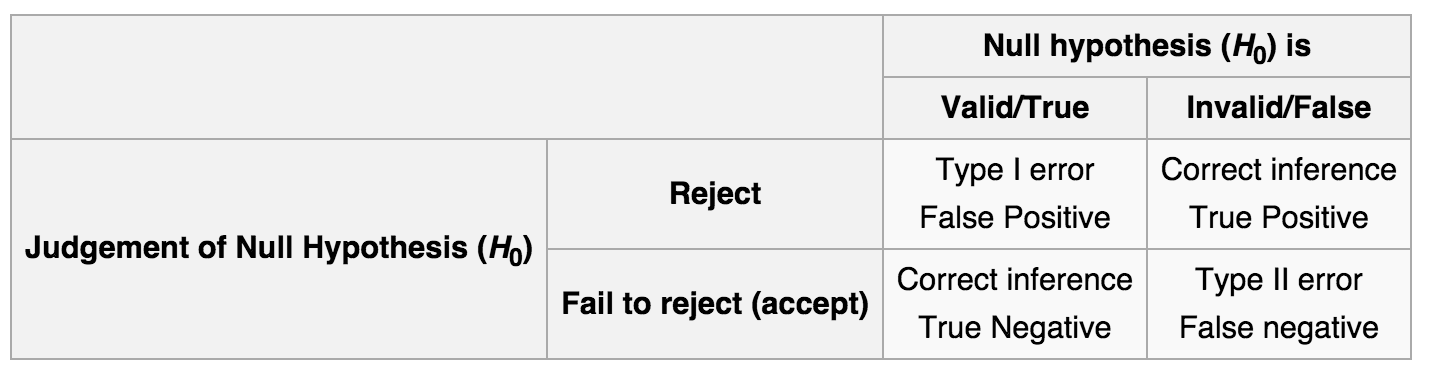
\includegraphics{hypothesis_testing.png}
\end{figure}

The rest of the paper is divided into four sections. 
The first section is devoted to cluster evaluation.
In the second section is about evaluation of 
machine translation systems. 
Next we move on to what are the right questions to ask and what comprises a good question. 
We conclude with a conclusion where I attempt to draw together twelve weeks and forty papers into four paragraphs.





\bibliography{scibib}

\bibliographystyle{Science}


\end{document}
